\documentclass[doublespacing]{bmcart}

\usepackage[colorlinks=true,linkcolor=black,citecolor=black,urlcolor=black]{hyperref}
\usepackage{amsmath,mathpazo}
\usepackage{comment,booktabs}
\usepackage{natbib,graphicx}
\usepackage{xspace,dcolumn}
\usepackage{setspace,upgreek}
\usepackage{siunitx,subcaption}
\doublespacing


%% SJE - commented these out for now.
%%\def\includegraphic{}
%%\def\includegraphics{}

\startlocaldefs
\newcommand{\um}{\,\ensuremath{\upmu \text{m}}\xspace}
\newcommand{\ournote}[1]{\marginpar{\textbf{#1}}}
\renewcommand{\ournote}[1]{}

\newcommand{\thref}[1]{\ref{#1}\marginpar{{\footnotesize
      {Table~\ref{#1} here}}}}
\newcommand{\fhref}[1]{\ref{#1}\marginpar{{\footnotesize
      {Fig.~\ref{#1} here}}}}

\newcommand{\ig}[1]{\centering\fbox{\includegraphics{#1}}}
\renewcommand{\ig}[1]{}
\providecommand*{\ped}[1]{\ensuremath{_\mathrm{#1}}}

\endlocaldefs

\begin{document}

\begin{frontmatter}

\begin{fmbox}

\dochead{Research}
\title{Emergence of correlated spontaneous activity in networks of stem-cell derived neurons}

\author[
   addressref={aff1},
   noteref={n1}
]{\inits{MKAK}\fnm{Muhammad Kaiser Abdul} \snm{Karim}}
\author[
   addressref={aff2},
   noteref={n1}
]{\inits{AS}\fnm{Alexander} \snm{Shtyrov}}
\author[
   addressref={aff1},
]{\inits{DST}\fnm{David S} \snm{Tourigny}}
\author[addressref={aff1},noteref={n2}]{
  \inits{MRNK}\fnm{Mark R N} \snm{Kotter}}
\author[addressref={aff1},noteref={n2}]{
  \inits{JSO}\fnm{John~S} \snm{O'Neill}}
\author[
   addressref={aff2},
   noteref={n2},
   email={sje30@cam.ac.uk}
]{\inits{SJE}\fnm{Stephen J} \snm{Eglen}}

\address[id=aff1]{
    \orgname{Department of Clinical Neurosciences and Wellcome Trust-MRC Cambridge Stem Cell Institute, University of Cambridge},
    \street{Cambridge Biomedical Campus},
    \city{Cambridge},
    \cny{UK}
}

\address[id=aff2]{
    \orgname{Department of Applied Mathematics and Theoretical Physics,
University of Cambridge},
    \street{Wilberforce Road},
    \city{Cambridge},
    \cny{UK}
}

\begin{artnotes}
\note[id=n1]{Equal contributor}
\note[id=n2]{Corresponding author}


\end{artnotes}

\end{fmbox}

\begin{abstractbox}

\begin{abstract}

We report the emergence of robust spontaneous activity in cultures of
neurons derived from IPSCs.  We tested the reproducibility of the recordings by repeating each recording three times from two different groups of neurons.  We find that spontanoues activity emerges after about 10 days of development.  As the cultures develop, more channels of the MEA detect activity.  

\end{abstract}

\begin{keyword}

\kwd{spontaneous activity}
\kwd{correlated activity}
\kwd{multielectrode arrays}

\end{keyword}

\end{abstractbox}

\subsection*{Abbreviations}
\begin{tabular}{ll}
  ISI & interspike interval\\
  IPSC & induced pluripotent stem cell\\
  MEA & multielectrode array\\
  DIV & days in vitro\\
  STTC & Spike Time Tiling Coefficent\\
\end{tabular}

\end{frontmatter}



\subsection*{Notes}
\textbf{Plan is to submit as a Short report to Neural Development:
  \url{https://neuraldevelopment.biomedcentral.com/submission-guidelines/preparing-your-manuscript/short-report}.
  An example of a recent short report can be found at 
\url{https://neuraldevelopment.biomedcentral.com/articles/10.1186/s13064-020-00140-y}}



\textbf{Kaiser: How shall we refer to developmental age -- DIV (days in
  vitro), DAP (days after plating) or other?}

\section*{Introduction}
State here the rationale for doing the recordings, and what we have
learnt.  (I like the J Neurosci ``3 paragraph model'': para 1 -
general idea, para 2 - what was done before, para 3 - what we did.  \textbf{Kaiser: would you be able to write the first two paragraphs?  I could say directly what we did for para 3 as a summary of the paper.})

\section*{Materials and Methods}

\subsection*{Data sets}
For recordings, MEAs incubated at \SI{37}{celcius}, 5\%
CO\textsubscript{2} were transferred to the MEA recording device
(MEA2100-2x60-System, Multichannel Systems). All recordings were
performed in atmospheric conditions with stage and custom-built heated
lid held at \SI{37}{celcius}. Developmental time course recordings took
place every second or third day, 10 min after a \SI{37}{celcius}, 5\%
CO\textsubscript{2} incubation following half-media change. MEAs were
allowed to equilibrate for 200 sec on the MEA recording device and
recording sessions lasted 10 min with local field potentials from all
electrodes sampled at 25 kHz.

\par There were two biological replicates, and three recording
sessions.  \textbf{TODO: discuss rationale for replicability.  How do we refer to the two types of reproducility -- there are the technical replicates (R1, R2, R3) and the biological replicates (2539, 2540).  Recordings started at about 7 days after plating, and then continued up until 40 days; for the last replicate we were able to extend the recording to 50 days.  (Perhaps say better why we went up to 50 days for the last replicate).}

\subsection*{Analysis}
\par The data were provided in a format written by MC\_DataTool \cite{Systems2014-tw}. The data were first converted to a data package based on the Frictionless Data Tabular Data Package specification \cite{Walsh2017-nm}. Each spike was represented by the time that the spike was detected. Conversion took place via our previous HDF5 format \cite{Eglen2014}.

\par After conversion the data were analysed using a series of Python
scripts to compute summary statistics and interspike intervals (ISIs),
carry out burst analysis, and extract network spikes. These scripts
make use of the Python \texttt{elephant} package
\cite{elephant_toolkit}.

\paragraph{Summary statistics} The summary statistics calculated were: population firing rate, number of spikes recorded, number of active channels, recording time, and firing rate per channel.

\paragraph{ISI histograms} ISIs were calculated for each channel in each recording. Histograms were plotted to show the distribution of ISIs. The bin width of the histograms was calculated by the recommended method in \texttt{matplotlib} \cite{Community2020-xp}. This computes the binwidth using two estimators: Freedman-Diaconis (bin width is inversely proportional to the cube root of the sample size) and Sturges (inversely proportional to the logarithm of the sample size). The minimum bin width of the two is then used.

\paragraph{Correlation} The spike time tiling coefficient (STTC) \cite{Cutts2014} was calculated for each pair of channels in each recording. A synchronicity window of 50 ms was used. The mean coefficient was plotted against age. Channels with an activity of less than 0.5 spikes per minute were excluded from STTC calculations as we found that these channels would otherwise produce unreliably high estimates of correlation.

\paragraph{Burst analysis} Burst analysis was carried out using an implementation of the MaxInterval method from NeuroExplorer, using the following parameters: a beginning ISI of 0.17 s, an end ISI 0.3 s, a minimum interburst interval (IBI) of 0.2 s, a minimum burst duration of 0.05 s, and a minimum of 3 spikes per burst. The parameters are those recommended in the NeuroExplorer manual \cite{neuroexplorer2020}. \textbf{Raster plots with bursts represented by coloured lines were produced. Box plots showing statistics of bursting behaviour over developmental time were also plotted. The statistics were: frequency of bursts, burst duration, firing rate in bursts, and \% spikes in bursts. Channels with an activity of fewer than 10 spikes per minute were excluded from bursting statistics.  This could be deleted/shortened, as we now don't show the bursting properties.}


\paragraph{Network spikes} Finally, network spikes were detected using a method similar to the one described by Eytan and Marom \cite{Eytan2006}. Spikes were placed in bins, with spikes occurring after the final bin discarded. The number of spikes in each bin was plotted. A network spike occurred when the number of action potentials in a bin exceeded one quarter of the total number of active channels. The 300 ms around the bin were extracted and plotted. Changing the bin width altered the number of detected network spikes, but heuristically it was found that bin widths below 10 ms or above 20 ms abrogated the shape of the extracted spike. Fixing the bin width at 20 ms, the number of network spikes was plotted against age.

\par Raster plots, plots of active channels, and plots of instantaneous firing rate against time were also produced from the raw data for comparison with the analysis of the data converted into the Frictionless format.


\paragraph{Computational environment} All data analysis were performed
in the Python programming language, version \textbf{...} on the linux operating system.

\paragraph{Availability of data and materials}


All data files and analysis code will be freely available from
\url{http://github.com/as2875/neurofrictionless.git}. \textbf{or
  similar repository}

\section*{Results}

\subsection*{Emergence of spontaneous activity in recordings}
We show the emergence of bursting activity (Figure~\ref{fig:rasters}).  These patterns were fairly typical across the different replicates although we have used quantitative methods in subsequent figures to highlight the changing properties of these recordings.

\subsection*{Simple measures of activity}
We can count the number of active electrodes, and total number of
spikes, population firing rate (and so on)
(Figure~\ref{fig:development}).

We did attempt to analyse the bursting structure of these spike
trains, although in line with our earlier work \cite{Cotterill2016-qi}
we found that finding burst detection parameters that worked across
all ages was difficult.  This became evident when we looked at the
distribution of interspike intervals on a log scale
(Figure~\ref{fig:bursts}).  Informally, for burst detection to work
well, we would expect to see at least a bimodal histogram, with the
first peak corresponding to intervals within a burst, and subsequent
peaks correponding to intervals between bursts (Figure 2C of
\cite{Charlesworth2015-gv}).  However, this was not observed often,
and so we decided not to further attempt to detect bursts in these
recordings.

\subsection*{Correlated activity}

Correlated activity is often seen in developing cultures of neurons
(refs).  To assess the correlations in the network, we have used the spike time tiling coefficient (STTC) \cite{Cutts2014}, which reports the correlation between pairs of spike trains: values of zero indicate that the trains are uncorrelated, whereas a value of +1 would indicate perfect correlation and negative values indicate anticorrelation.  This tends to occur days/weeks after individual neurons have
begun firing, and may reflect the development of connectivity between
neurons.  In all our cultures, although there was spontaneous activity
from about day 10, correlated activity was often not observed until
day 18-20 partly due to the low firing rates of individual channels
(asterisks in Figure~\ref{fig:correlation}.  After about day 18-20,
however, we see that spike trains are correlated across the array; no
strong developmental trend was observed.  We could see however that
when correlations were found in a recording, there was often a bimodal
structure, with groups of highly correlated neurons and uncorrelated
(as shown in the violin plots of Figure~\ref{fig:correlation}.  We did not observe any significant anticorrelations in our recordings.

\subsection*{Network spikes}
Network-level activity ramps up over time, although there are some
cultures that do not generate network spikes as late as DIV 40.
(Figure~\ref{fig:networkfreq}).

\section*{Discussion}
\textbf{Discuss in context of Frega study}  \cite{Frega2019}

\textbf{This may need only be a couple of paragraphs}

Overall the reproducibility of the recordings was high, with only one recording (R2 of 2540) possibly showing less correlated activity than the other recordings.

\vspace*{1cm}

\begin{backmatter}

\subsection*{Acknowledgements}


\textbf{Kaiser: what funding do you need to acknowledge?}  This work was supported by a Frictionless Data grant to SJE\@.  Thanks
to Dr Lilly Winfree from Frictionless Data for her feedback on the
project.


\bibliographystyle{vancouver}
\bibliography{ipsc20}

\clearpage
\section*{Figures}
\begin{figure}[h!]
  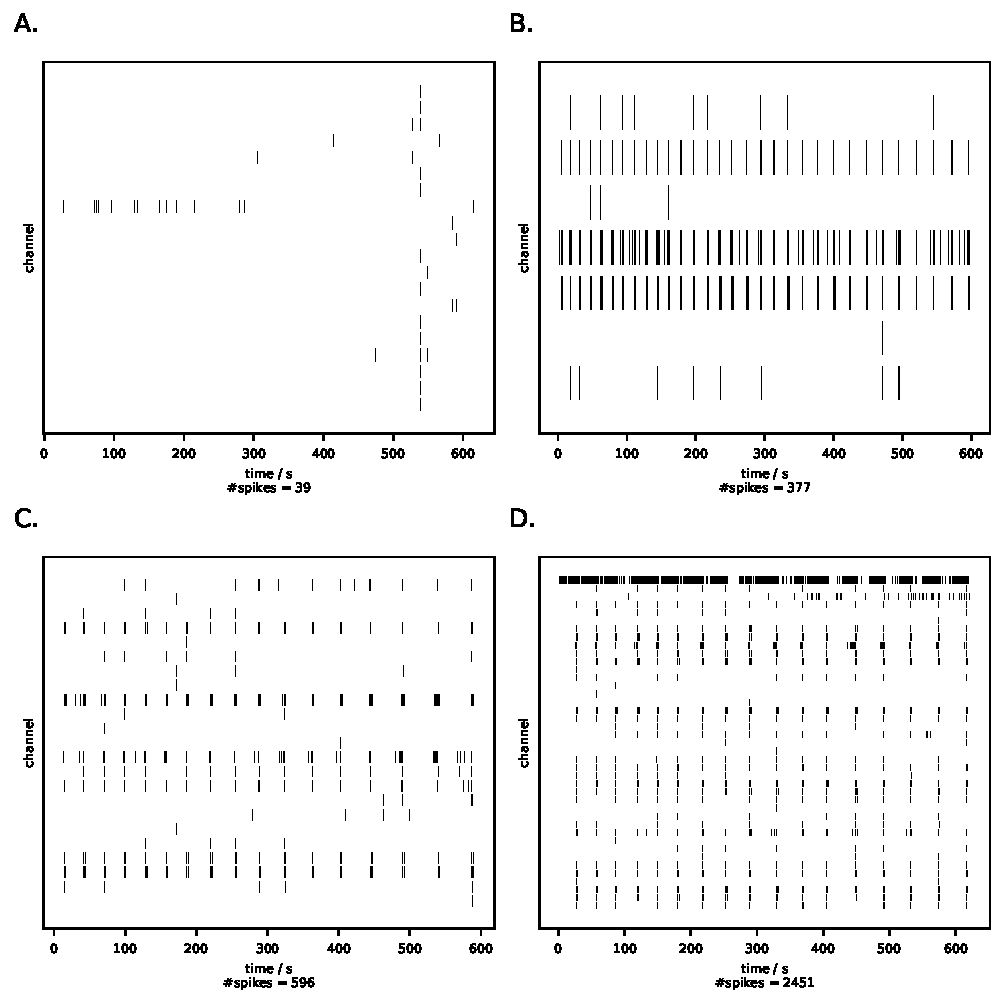
\includegraphics{../plots/supplementary_figures/raster_plots.pdf}
  \caption{Emergence of spontaneous activity in a population of neurons. Representative recordings from the first series (R1) on replicate 2540 are shown at four ages. All spikes captured during the recording interval are displayed for each age.  Scale bar in top-left denotes 20 seconds and applies to all rasters.}
  \label{fig:rasters}
\end{figure}

\begin{figure}[h!]
    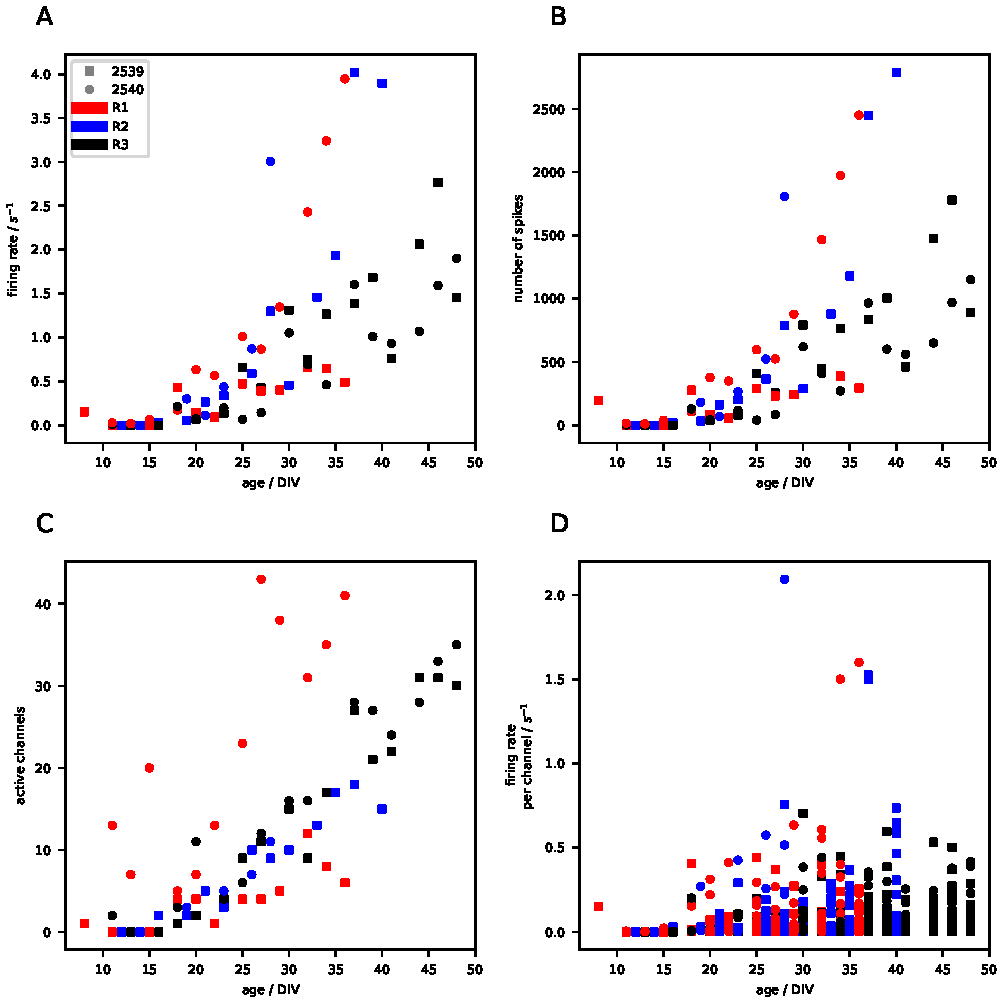
\includegraphics{../plots/development_plots.pdf}
	\caption{Firing of neurons over time after plating. The metrics shown are (A) population firing rate, (B) firing rate of individual channels and (C) number of active channels, defined as the number of channels with at least one recorded spike.  In each panel, the shape of the symbol reflects the biological replicate, and the colour of each symbol represents the technical replicate, as shown in the legend of panel A. \textbf{AS: y axis in each case should not drop below 0.0}}
	\label{fig:development}
\end{figure}


%% Extracted page 44 using:
%% pdftk logisi_plots.pdf cat 44 output logisi_plot44.pdf
\begin{figure}[h!]
  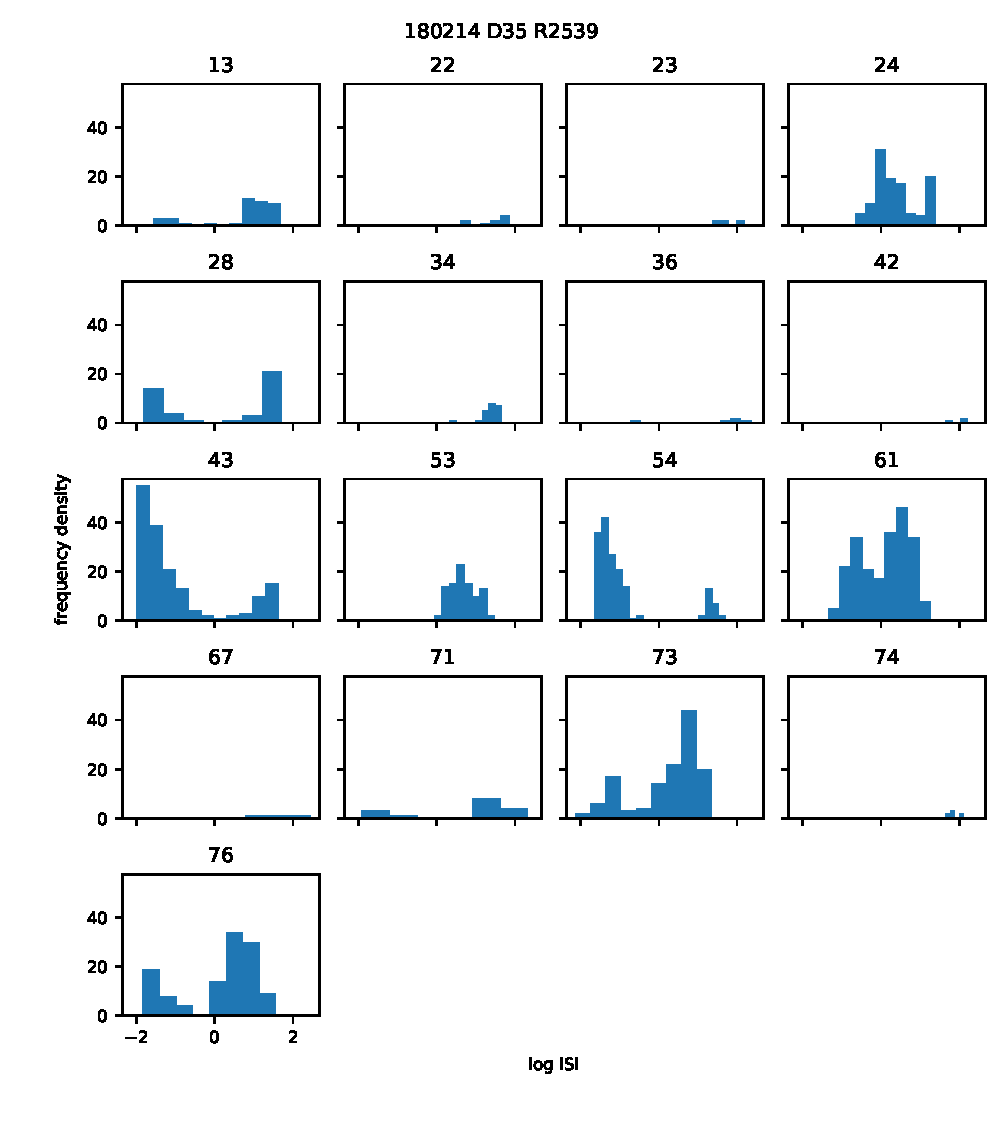
\includegraphics{../plots/logisi_plot44.pdf}
	\caption{Distribution of interspike intervals. Each plot shows the frequency distribution of the log interspike interval from each  channel (written above each histogram) of one recording (R2539, D18).  The x axis is the log (base 10?) of the interspike interval and the y axis is the count.  \textbf{The bin width of each histogram is selected by an adaptive algorithm, described in Methods.  Can you try to convert the x axis labels to sensible time values (0 to 1 second? -2 to 0.01 second; +2 to 100 seconds)}}
	\label{fig:logisi}
\end{figure}

\begin{figure}[h!]
    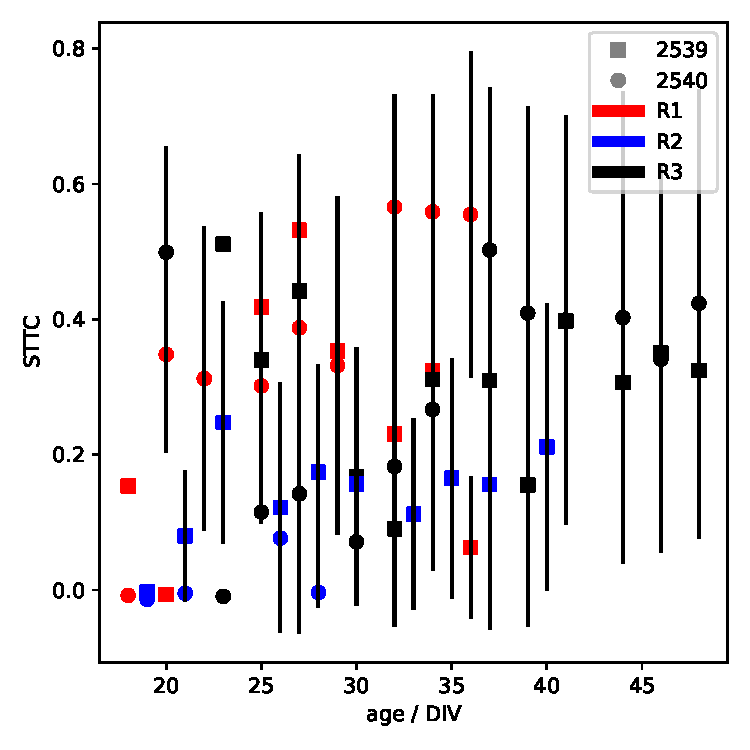
\includegraphics{../plots/correlation_plots.pdf}
	\caption{Violin plots of channel correlations over time. The STTC was used as the measure of spike train correlation. STTCs were calculated pairwise on the set of channels with activities above a threshold. A low threshold of 0.5 \(\text{min}^{-1}\) was used in this analysis, and recordings with no channels above the threshold are represented by an asterisk. The small number above each distribution is the number of STTCs in the distribution. The bars represent the absolute range of values.}
	\label{fig:correlation}
\end{figure}

\begin{figure}[h!]
    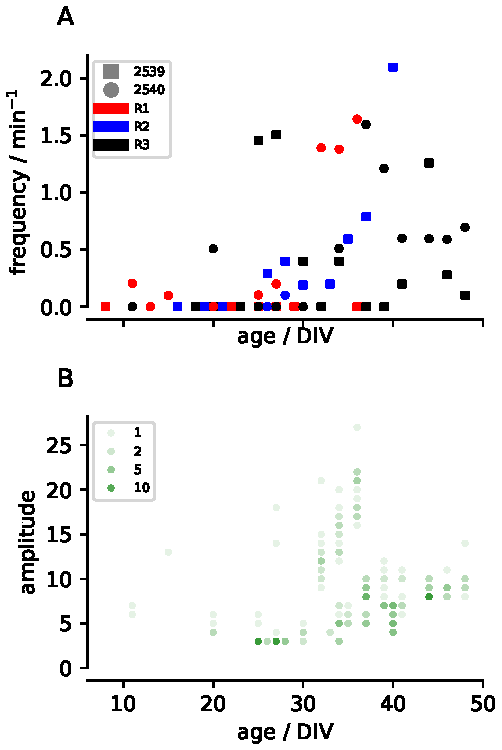
\includegraphics{../plots/network_spikes_scatter.pdf}
	\caption{Quantification of network spikes across development. No channels were discarded when detecting network spikes. (A) Frequency of occurrence of network spikes over time. (B) Amplitude of network spikes, defined as the number of spikes in the bin representing the peak of the network spike. All recordings in the dataset are shown on this plot. The opacity of each point is proportional to the number of network spikes lying at that point on the graph.  \textbf{AS: the y axis in A should not go below 0.0, as it is a frequency; in B, we should probably draw the y axis starting from 0.}}
	\label{fig:networkfreq}
\end{figure}

\end{backmatter}

\end{document}

%% LocalWords: Eglen MEA





